\renewcommand{\S}{\mathcal{S}}
\newcommand{\A}{\mathcal{A}}
\newcommand{\R}{\mathcal{R}}
\newcommand{\M}{\mathcal{M}}
\renewcommand{\P}{\mathbb{P}}
\renewcommand{\E}{\mathbb{E}}

\chapter{Reinforcement Learning}\label{Ch:Reinforcement Learning}

In this chapter, we introduce the fundamental concepts of reinforcement learning algorithms. We start with a broad overview of reinforcement learning and dive into the basic principles of Markov Decision Processes, Value Functions, Bellman Optimality Equations and Temporal Difference Learning. 

\section{Reinforcement Learning Overview}\label{sec1}
\begin{figure}[h!]
\centering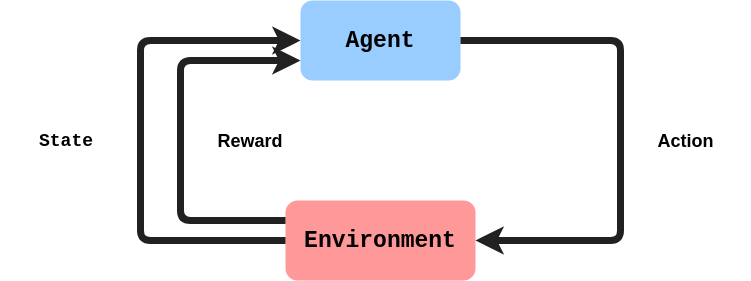
\includegraphics[scale=0.5,clip]{Graphics/RL_1.png}
\caption{Interaction of Agent and Environment}
\label{fig:RL_overview}
\end{figure}

Following \textit{Reinforcement Learning} by Sutton and Barto \cite{sutton1998reinforcement}, we define Reinforcement Learning as the field dedicated to the study of the Reinforcement Learning Problem (RLP). The Reinforcement Learning Problem can be defined broadly as the problem of learning from interaction to achieve a goal. The decision maker is called the \textit{agent}, while the world it interacts with is called the \textit{environment}. These two interact continually: the agent acts and the environment responds accordingly, presenting new situations to the agent. The environment also provides feedback to the agent via a scalar \textit{reward} signal. The goal of reinforcement learning is to learn a strategy, called \textit{policy}, that maximizes the expected cumulative reward the agent can receive. This process is illustrated in Figure \ref{fig:RL_overview}. In the following sections, we base our treatment of the material on \cite{szepesvari2010algorithms}. 

\section{Markov Decision Processes}\label{sec2}
The mathematical framework used to study the RLP, is the theory of Markov Decision Processes (MDPs), which allows for the modeling of sequential decision-making processes, subject to Markovian conditional independence assumptions. Here we restrict ourselves to countable MDPs, however there exist extensions to continuous state-action MDPs too. 

\begin{definition}
A Markov decision process is a tuple $ ( \S, \A, \P, \gamma) $ where
\begin{enumerate}
  \item $\S$ is a finite set of states
  \item $\A$ is a finite set of actions
  \item $\P := \P\left(S_{t+1} = \cdot, R_{t+1} = \cdot \mid S_t = \cdot,\ A_t = \cdot \right) : \S \times \mathbb{R} \times \S \times \A \rightarrow [0,1]$ is the state   transition probability matrix
  \item $\gamma \in [0,1]$ is the discount factor
\end{enumerate}
\end{definition}

Given an MDP $\M$, the interaction between the agent and its environment happens as follows: Let $t \in \mathbb{N}$ denote the current time, and let $S_t$ and $A_t$ denote the state of the environment and the action selected by the decisionmaker, respectively.  Upon receiving the action chosen by the agent, the environment makes a transition according to the dynamics of $\P$:
\begin{align}
  \left( S_{t+1}, R_{t+1} \right) \sim \P\left( S_{t+1} = \cdot, R_{t+1} = \cdot \mid S_t, A_t \right)
\end{align}

\begin{definition}
A policy $\pi \left( \cdot \mid \cdot \right) : \A \times \S \rightarrow [0,1]$ is a conditional probability distribution over actions, given the state. 
\end{definition}

Note that the policy fully defines the behavior of the agent. The last notion we need to define the problem is the \textit{return}.

\begin{definition}
The return underlying a policy $\pi$ is defined as the total discounted sum of the rewards incurred:
\begin{align}
  \R = \sum\limits_{t=0}^{\infty} \gamma^{t} R_{t+1}
\end{align}
\end{definition}

The goal of the agent is to learn a policy that performs well. Our measure of performance is the \textit{expected return}--a rather natural metric. 

\section{Value Functions}\label{sec3}
Given the expected return characterization of performance, we can compare two policies and decide which one leads to better rewards. But how do we find good policies? The optimal value $V^* (s)$ of $s \in \S$ is the highest achievable expected return when the process is started from state $s$. We call $V^*:\S \rightarrow \mathbb{R}$ the optimal value function, and if a policy $\pi_*$ achieves these optimal values in all states, it is called an \textit{optimal policy}. We can extend the notion of value function to arbitrary policies: 

\begin{definition} The value function $V^{\pi} : \S \rightarrow \mathbb{R}$ underlying the policy $\pi$ is defined as
\begin{align}
  V^{\pi} \left( s \right) = \E \left[ \R \mid S_0 = s \right] = \E \left[\sum\limits_{t=0}^{\infty} \gamma^{t} R_{t+1} \mid S_0 = s \right]
\end{align}
where the values $R_{t+1}$ are obtained following policy $\pi$. 
\end{definition}

A related object is the action-value function of a policy $\pi$. 

\begin{definition} The action-value function $Q^{\pi} : \S \times \A \rightarrow \mathbb{R}$ underlying the policy $\pi$ is defined as
\begin{align}
  Q^{\pi} \left( s, a \right) = \E \left[ \R \mid S_0 = s, A_0 = a \right] = \E \left[\sum\limits_{t=0}^{\infty} \gamma^{t} R_{t+1} \mid S_0 = s, A_0 = a \right]
\end{align}
where the values $R_{t+1}$ are obtained following policy $\pi$. 
\end{definition}

Similar to the way we defined $V^*$, we can define the optimal action-value function $Q^*$, given to rise by the optimal policy $\pi_*$. Due to the Markov property, given $V^*$ and $\P$, we can easily devise an optimal policy: in a given state, choose the action that leads to maximal average $V^*$ value. With Q we can do even better: Given just $Q^*$, the policy $\pi(s) = \arg\max\limits_{a \in \A} Q^*(s, a)$ is optimal. Note that in the MDPs considered here, an optimal policy always exists. 

\section{Bellman Optimality Equations}\label{sec4}
Denote $r(s,a) := \E \left[ R_{t+1} \mid S_t = s,\ A_t = a \right]$. Then the optimal value function $V^*$ and $Q^*$ are connected by the following equations: 
\begin{align}
V^* (s) &= \sup\limits_{a \in \A} Q^* (s, a) \label{eq:V-opt-simple} \\
Q^* (s, a) &= r(s,a) + \gamma\ \E\left.\left[ V^* \right| S_t=s,\ A_t=a \right] \label{eq:Q-opt-simple} \\
&=  r(s,a) + \gamma\ \sum\limits_{w \in \S} \P \left( S_{t+1}=w \mid S_t = s,\ A_t = a \right) V^*(w)\\
\end{align}

These can be shown to hold by simple conditioning arguments. Intuitively they can be thought of as saying the following: Suppose we are following an optimal policy $\pi_*$. By optimality, in state $s$, we must choose an action with maximal state-action value $Q^*$. But then it must be that $V^*$ is equal to this maximal value, and Equation (\ref{eq:V-opt-simple}) follows. Equation (\ref{eq:Q-opt-simple}) follows by a similar argument. Combining these two equations gives rise to the Bellman Optimality Equations: 
\begin{align}
V^* (s) &= \sup\limits_{a \in \A} \left\lbrace  r(s,a) + \gamma\ \sum\limits_{w \in \S} \P \left( S_{t+1}=w \mid S_t = s,\ A_t = a \right) V^*(w) \right\rbrace \label{eq:V-opt} \\
Q^* (s, a) &=  r(s,a) + \gamma\ \sum\limits_{w \in \S} \P \left( S_{t+1}=w \mid S_t = s,\ A_t = a \right) \sup\limits_{a \in \A} Q^* (w, a) \label{eq:Q-opt}
\end{align}

A short proof of Equation (\ref{eq:Q-opt}) is given in the next section. Introducing new notation, we can rewrite Equation (\ref{eq:V-opt}) more succinctly, in a way that suggests a solution:

\begin{definition}
Define the Bellman Optimality operator $T^*: \mathbb{R}^\S \rightarrow \mathbb{R}^\S $, by
\begin{align}
(T^*V)(s) = \sup\limits_{a \in \A} \left\lbrace  r(s,a) + \gamma\ \sum\limits_{w \in \S} \P \left( S_{t+1}=w \mid S_t = s,\ A_t = a \right) V(w) \right\rbrace
\end{align}
Then the Bellman Optimality Equation for V can be rewritten as 
\[
T^*V^* = V^*
\]
\end{definition}

An analogous operator exists for $Q^*$ that we don't cover here. Under certain conditions, it can be shown that both (nonlinear) Bellman Optimality operators are in fact contractions. Thus, by a fixed point argument, they have unique solutions that can be iteratively approximated. Such iterative approximations have been the bases of many of the early reinforcement learning algorithms. 

\section{Temporal Difference Learning}\label{sec5}
Instead of pursuing these fixed point approximation methods, we turn to the more sophisticated Temporal Difference (TD) Learning approach, one of the most significant ideas in reinforcement learning. Recall the optimality equation for $Q^*$:
\begin{align}
Q^*(s_t, a_t) &= \E\left.\left[R_{t+1} + \gamma R_{t+2} +
\gamma^2 R_{t+3} + \cdots = \sum_{i=t}^{\infty} \gamma^{i-t}R_{i+1}
\right| S = s_t, A = a_t \right] \\
&= \E\left.\left[R_{t+1} + \E\left.\left[ \sum_{i=t + 1}^{\infty} \gamma^{i-t}R_{i+1}
\right| s_t, a_t, S_{t+1} \right] \right| S = s_t, A = a_t \right] \nonumber \\
&\stackrel{*}{=} \E\left.\left[R_{t+1} + \gamma\ \max\limits_{a' \in \A} \E\left.\left[ \sum_{i=t + 1}^{\infty} \gamma^{i-(t + 1)}R_{i+2}
\right| S_{t+1}, A_{t+1}=a' \right] \right| S = s_t, A = a_t \right] \nonumber \\
&= \E\left.\left[R_{t+1} + \gamma\ \max\limits_{a' \in \A} Q^*(S_{t+1},a') \right| S = s_t, A = a_t \right] \label{eq:Q-optimality}
\end{align}

where the starred equality follows by the Markov property and the fact that we follow the optimal policy $\pi_*$. This splits $Q^*$ into two quantities: the immediate reward and the discounted
future rewards. More importantly,
Equation (\ref{eq:Q-optimality}) reveals structure that 
immediately yields a suitable iterative update shown in Equation (\ref{eq:q_iter_up}).
\begin{align}\label{eq:q_iter_up}
Q(s_t, a_t)_{j+1} &= Q(s_t, a_t)_j + \alpha \;
\left(R_{t+1} + \gamma \; \underset{a'}\max \; Q(s_{t+1},a') - Q(s_t, a_t)\right)
\end{align}
where $\alpha \in [0, 1]$. As $\alpha$ approaches 1, 
the $Q$ value function is constructed to weight the 
future rewards more heavily. 

This update is in the standard iterative update format
$Q(s_t, a_t)_{j+1} = Q(s_t, a_t)_j + \alpha \times \textrm{error} $ where
the error captures the difference between what the value $Q(s_t, a_t)$ 
\textit{should} 
be at the current iteration: $R_{t+1} + \gamma \; \underset{a' \in \A}\max \; Q(s_{t+1},a')$ 
and what it is at the current iteration: $Q(s_t, a_t)$. 

In the next section we expand on this idea, and introduce the Q-learning algorithm, which will form the basis of our investigations. 
\endinput


